\section{Creación del primer paquete DTSX}

1. Abriremos un nuevo Proyecto en nuestro Visual Studio.
	\begin{center}
	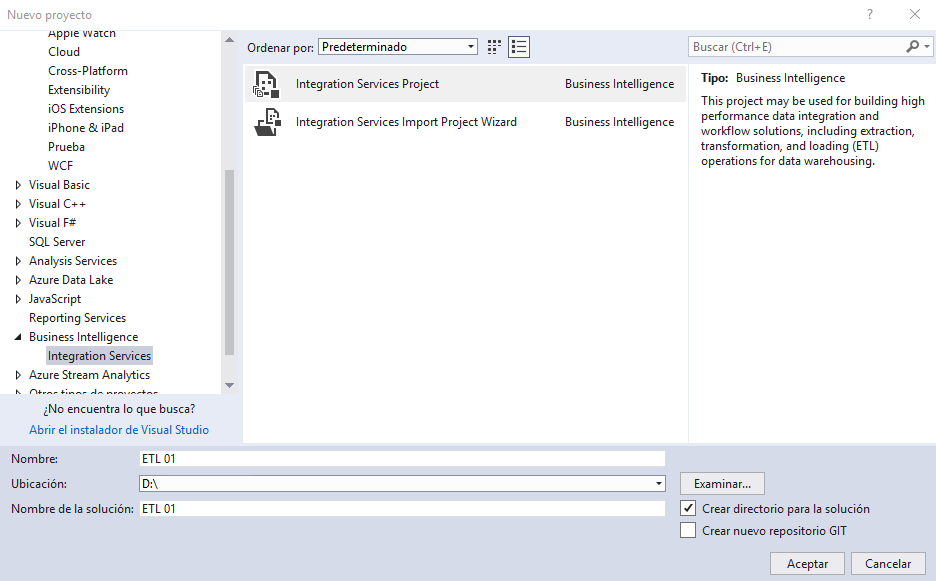
\includegraphics[width=10cm]{imagenes/img13}
	\end{center}	

2. En al ventana nueva, sección Solución Explorer, Agrego el paquete generado antes.
	\begin{center}
	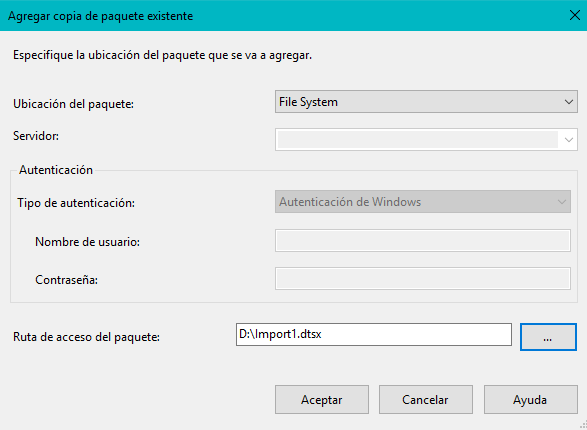
\includegraphics[width=10cm]{imagenes/img14}
    \end{center}	
    
	\begin{center}
	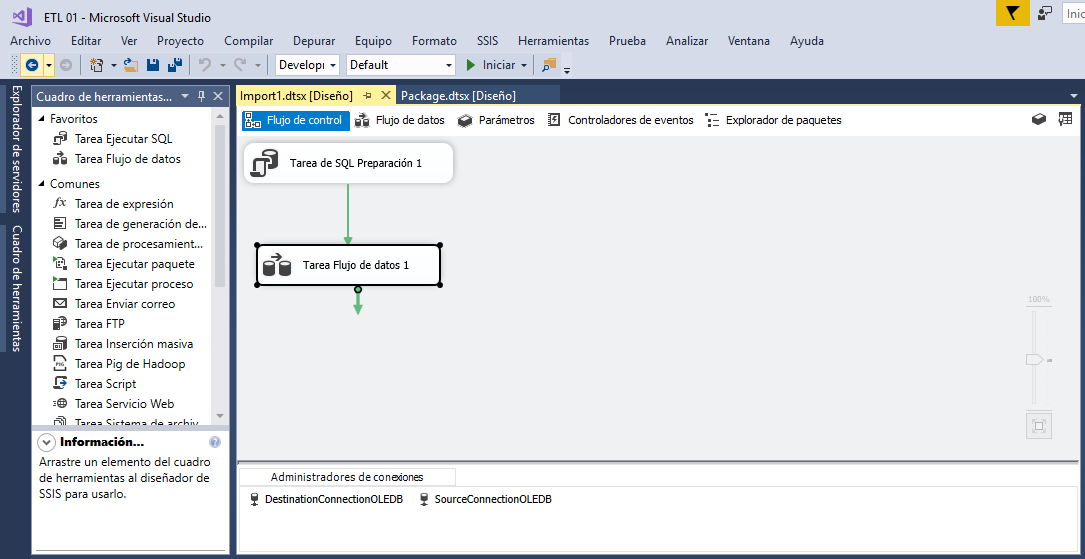
\includegraphics[width=10cm]{imagenes/img15}
    \end{center}	
    
	\begin{center}
	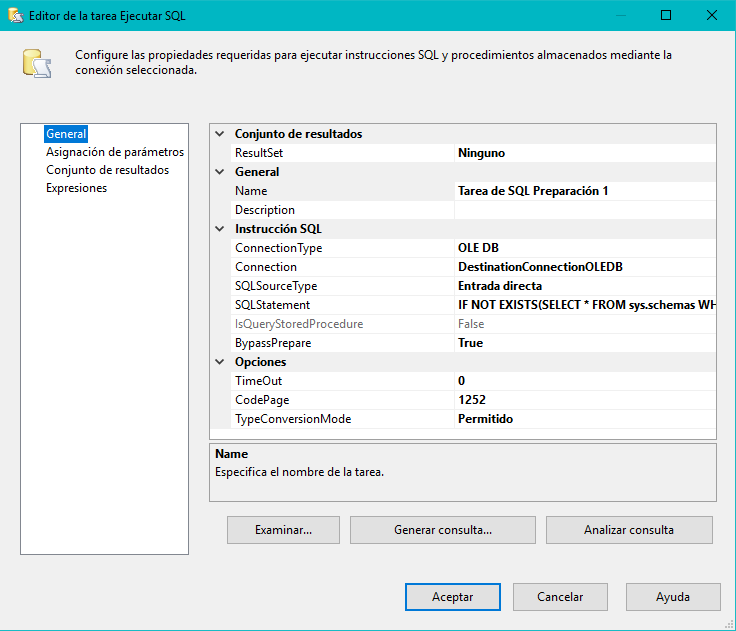
\includegraphics[width=10cm]{imagenes/img16}
	\end{center}	

3. En la siguiente ventana mostramos el paquete que se ha importado.
	\begin{center}
	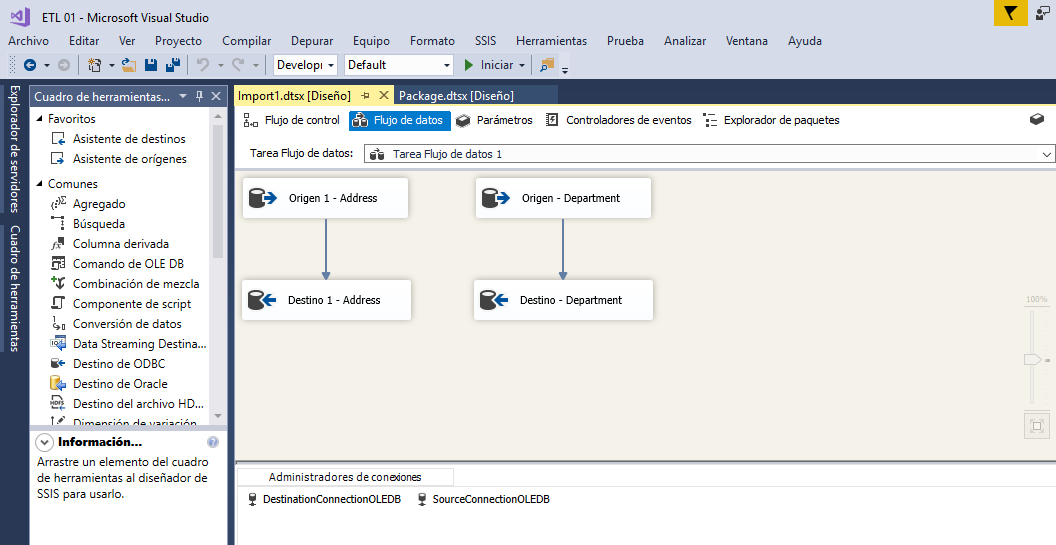
\includegraphics[width=10cm]{imagenes/img17}
    \end{center}	
    
	\begin{center}
	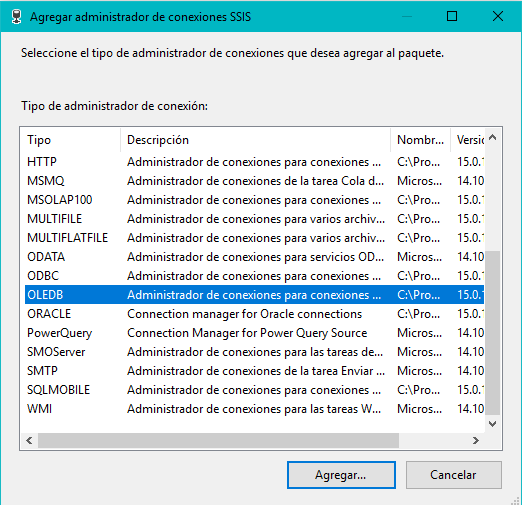
\includegraphics[width=10cm]{imagenes/img18}
	\end{center}	

4. En la siguiente ventana mostramos el paquete que se ha importado.
	\begin{center}
	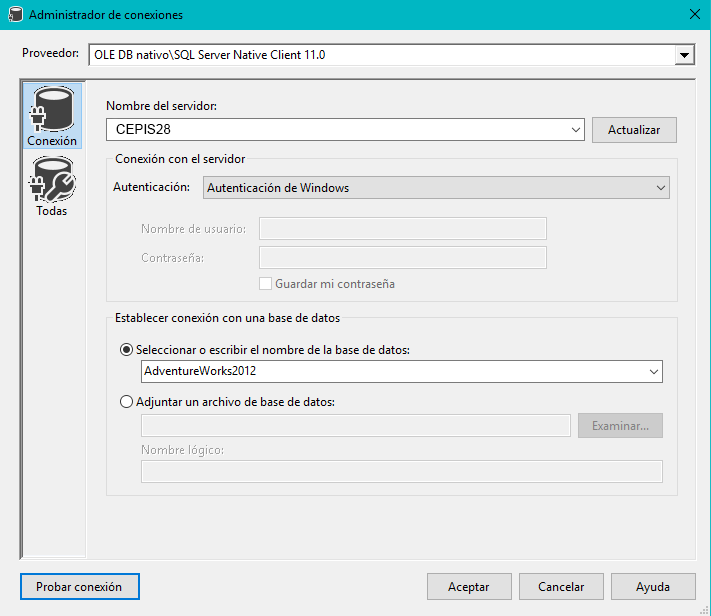
\includegraphics[width=10cm]{imagenes/img19}
    \end{center}	
    
	\begin{center}
	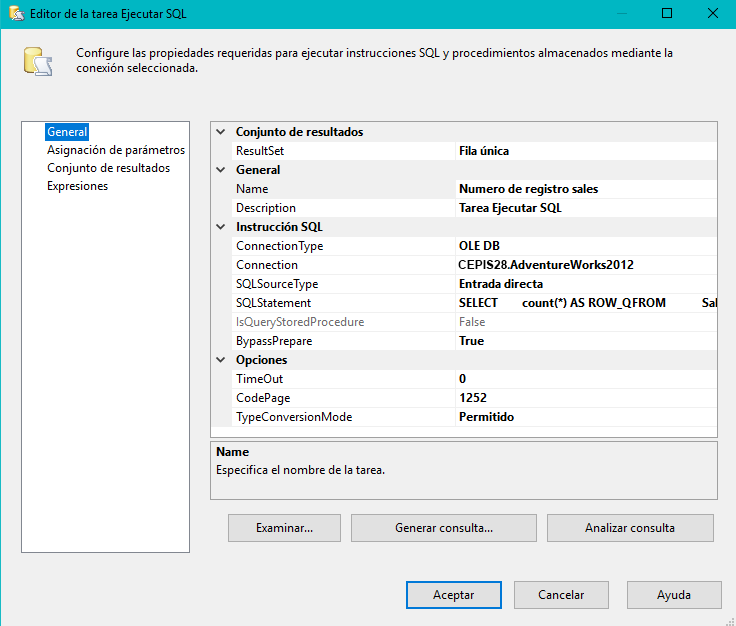
\includegraphics[width=10cm]{imagenes/img20}
	\end{center}	
	

5. Editamos el componente Scrtipt Task Editor.
    \begin{center}
	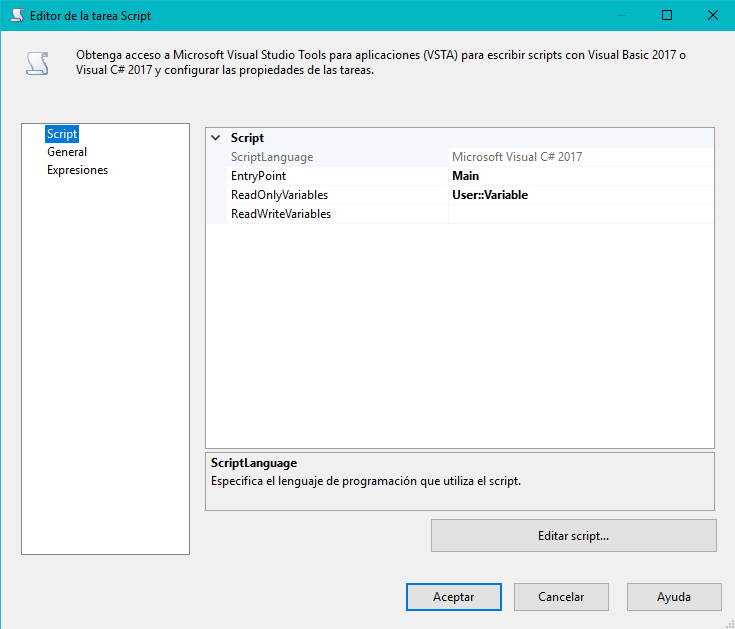
\includegraphics[width=10cmh]{imagenes/img21}
    \end{center}	
    
	\begin{center}
	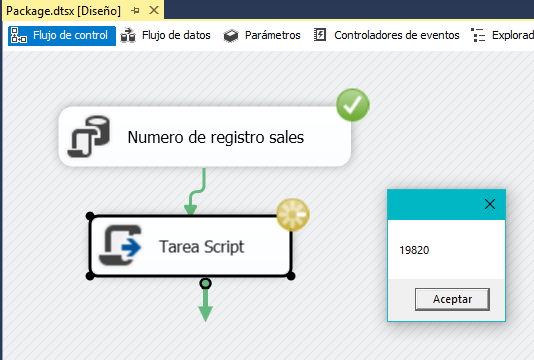
\includegraphics[width=10cm]{imagenes/img22}
    \end{center}	
    
	\begin{center}
	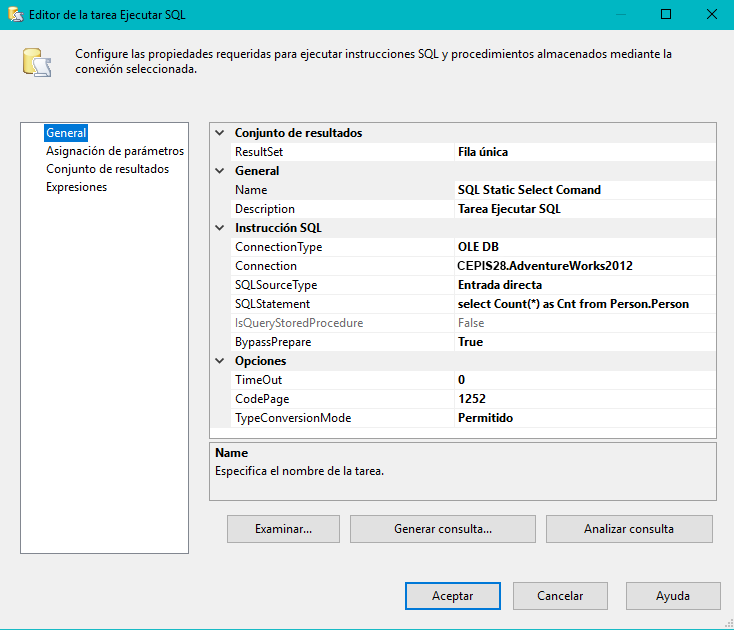
\includegraphics[width=10cm]{imagenes/img23}
    \end{center}	
    
	\begin{center}
	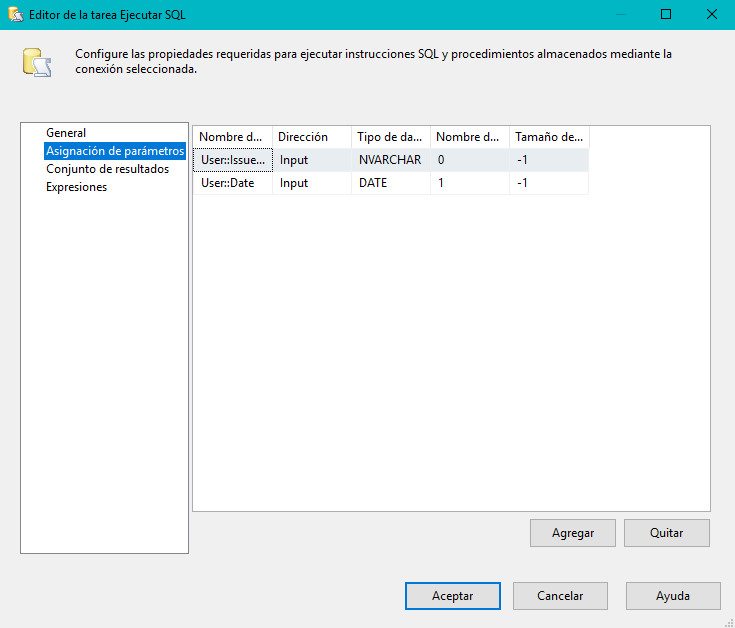
\includegraphics[width=10cm]{imagenes/img24}
    \end{center}	
    
	\begin{center}
	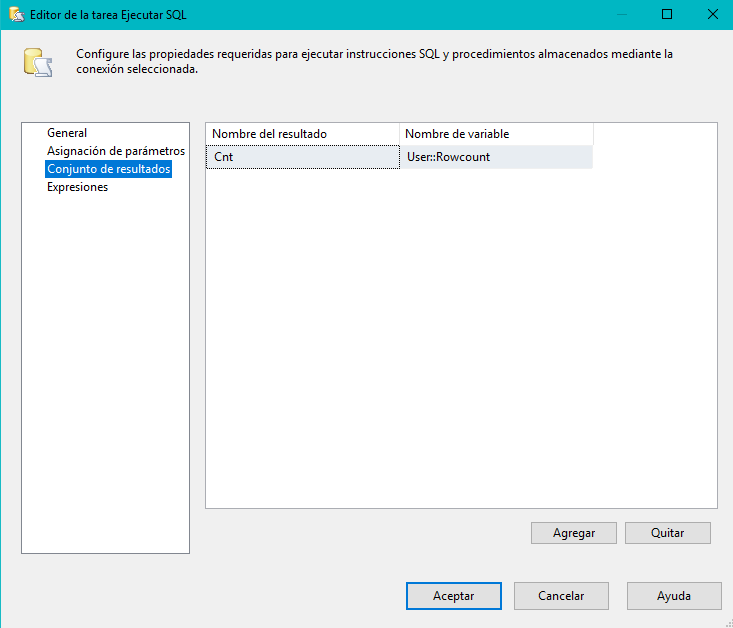
\includegraphics[width=10cm]{imagenes/img25}
    \end{center}	
    
	\begin{center}
	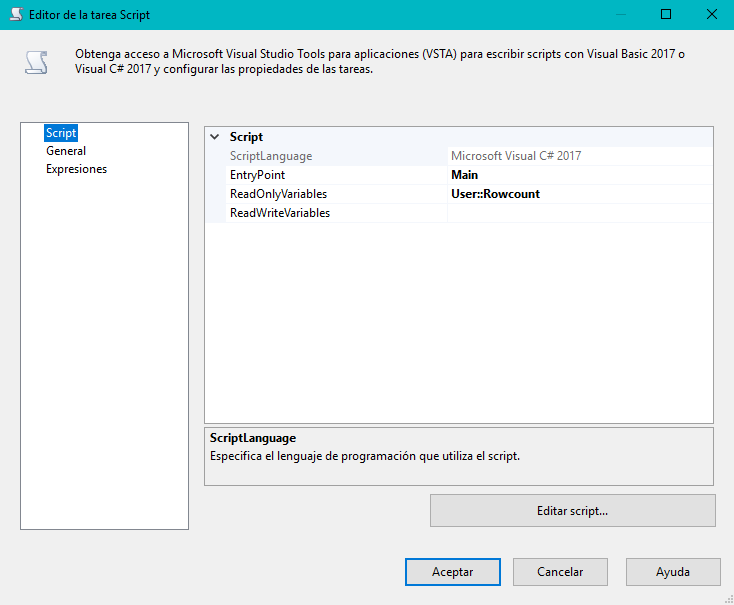
\includegraphics[width=10cm]{imagenes/img26}
    \end{center}	

6. Guardamos y los ejecutamos.
    \begin{center}
	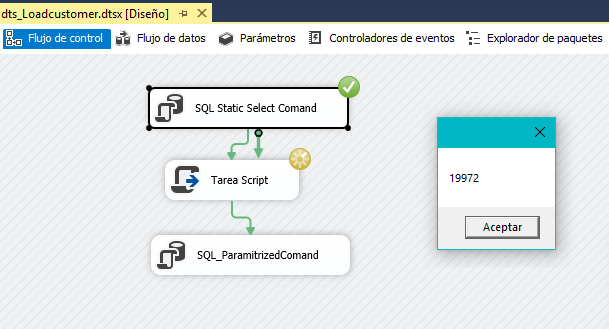
\includegraphics[width=10cm]{imagenes/img27}
	\end{center}	